\chapter{Fundamentação Teórica}\label{ch:teoria}
Neste capítulo, serão levantados dados sobre a necessidade de meios para combater a escassez global da produção de alimentos, sendo abordados detalhes técnicos da área de atuação deste \textit{software}, que é voltado à pesquisas e experimentos na área da Agronomia, sobre a qualidade do solo e suas atividades enzimáticas para um melhor aproveitamento do solo na produção de alimentos. Além disso, serão discutidos pontos referentes ao crescimento da mobilidade no Brasil e no mundo, trazendo o contexto da solução apresentada por este projeto, bem como conceitos técnicos relacionados aos dispositivos móveis, desenvolvimento de \textit{software}, metodologias ágeis e arquitetura do sistema.

\section{Qualidade do solo}\label{sec:qualidade_solo}
A \ac{qs} é um dos fatores fundamentais para o aumento da produtividade agrícola e, consequentemente, para a redução da escassez global de alimentos. Segundo a \ac{fao}, cerca de um terço dos solos do mundo estão degradados devido a práticas agrícolas insustentáveis e outros fatores como poluição, erosão, compactação e perda de matéria orgânica. Além disso, a \ac{onu}\footnote{\ac{onu} - População: \url{https://www.un.org/en/global-issues/population}} estima que a população mundial chegará a 9,7 bilhões em 2050, o que exigirá um aumento de 70\% na produção de alimentos para suprir a demanda crescente \citet{fao2018future}.

Nesse contexto, é fundamental entender a \ac{qs}, suas características físicas, químicas e biológicas, bem como as interações entre esses fatores. Isso permitirá o desenvolvimento de técnicas mais eficientes e sustentáveis de manejo do solo, contribuindo para a melhoria da produtividade agrícola e, consequentemente, para a redução da escassez global de alimentos.

Desta forma, trazendo o problema para o escopo do Brasil, surge a necessidade de conciliar nossa produção agrícola com a preservação ambiental, e isso têm despertado a atenção da comunidade científica e os produtores para a necessidade de associar produtividade e formas mais sustentáveis de produção \citet{lopez2019carbon}. Com este objetivo, as medidas da \ac{cnd} acordada pelo Brasil com a Convenção Quadro das Nações Unidas sobre mudanças climáticas, incluem como estratégia o fortalecimento do \ac{planoabc} através do desenvolvimento sustentável na agricultura até 2030 \citet{embrapa_visao_2030}.

\section{Cálculo de atividades enzimáticas do solo}\label{sec:calculo_enzimatico}
Diversos métodos são utilizados para avaliar a qualidade do solo, como a análise físico-química, a análise da comunidade microbiana do solo e a \ac{ae} do solo. Esta última pode ser utilizada como uma medida da atividade biológica do solo, pois as enzimas são produzidas pelos microrganismos presentes no solo e são essenciais para a decomposição da matéria orgânica, a liberação de nutrientes e a formação de compostos benéficos para as plantas.

O cálculo de \acp{ae} do solo é uma importante ferramenta para avaliar a qualidade e saúde do solo, uma vez que a atividade enzimática está diretamente relacionada com a quantidade e diversidade de microrganismos presentes no solo. Alguns exemplos de enzimas que respondem quanto a qualidade do solo são a fosfatase ácida, a $\beta$-glucosidase, a urease e a protease. A atividade dessas enzimas pode ser afetada por vários fatores, como o pH do solo, a umidade, a temperatura e a presença de metais pesados. Portanto, a análise das \acp{ae} do solo é importante para identificar possíveis impactos ambientais e planejar práticas de manejo sustentável \cite{agrogalaxy}.

% Existem diversas metodologias para o cálculo dessas \acp{ae}, incluindo ensaios espectrofotométricos, cromatográficos e fluorimétricos. Além disso, é importante considerar fatores como a temperatura e pH ideais para cada enzima, bem como a influência de diferentes tipos de solo e uso da terra na \ac{ae}.

Entre as referências bibliográficas relevantes para o estudo de \acp{ae} em solo, podemos citar o trabalho de \citet{tabatabai1969use}, que desenvolveram uma metodologia para a determinação de fosfatase ácida em solo; o estudo de \citet{ribeiro2019atividade}, que avaliou a atividade das enzimas fosfatase ácida e alcalina e $\beta$-glicosidase como indicadores da qualidade do solo em uma área de plantio da Embrapa Milho e Sorgo, destacando diferenças entre o solo cultivado e o solo de cerrado natural, sugerindo a necessidade de práticas de manejo para recuperação biológica do solo; o estudo de \citet{allison2010measurement}, que comparou diferentes metodologias para a medição da \ac{ae} em solos de diferentes ecossistemas; e o trabalho de \citet{sinsabaugh2008stoichiometry}, que avaliou a influência da qualidade do substrato e da umidade do solo na atividade enzimática.

\section{Mobilidade}\label{sec:mobilidade}
Segundo \citet{b2004mobile}, um sistema de computação móvel é um sistema que pode ser facilmente movido fisicamente ou cuja funcionalidade pode ser usada durante o movimento. Como esses sistemas fornecem essa mobilidade, essas funcionalidades adicionadas são a razão para caracterizar separadamente os sistemas de computação móvel, eles geralmente oferecem capacidades e recursos não encontrados em sistemas normais, como: 
 \begin{itemize}
   \item Armazenamento de dados local e/ou remoto via conexões com ou sem fio;
   \item Segurança para persistência de dados em caso de queda de energia ou pane;
   \item Sincronização de dados com outros sistemas.
 \end{itemize}

Atualmente, pensamos em um sistema móvel como um sistema projetado para rodar em um computador de mão, seja ele celular, tablet ou qualquer outro dispositivo com tais características. Pela definição acima, os notebooks também são considerados plataformas para sistemas móveis, mas não são utilizados exatamente da mesma forma que os dispositivos citados acima, pois é necessário parar em algum lugar, abrir o notebook, esperar carregar, etc...

\section{Dispositivos móveis}\label{sec:dm}
Para adentrar no universo da solução apresentada, os \acp{dm}, é valioso abordar como estes \textit{gadgets} lidam com a capacidade de armazenamento e processamento de dados, que, por possuírem sistemas móveis espera-se que os mesmos possuam menor eficiência para desenvolver atividades se comparados a um computador estacionário (\ac{pc}), por exemplo, que possui muito mais disponibilidade energética para realizar suas tarefas, porém, nos dias de hoje esse \textit{gap} para atividades cotidianas está mais estreito, devido aos grandes avanços da tecnologia voltados a este segmento que vem em forte alta — o qual, segundo \citet{data.ai} cresceu 20\% em 2020 comparado ao ano anterior, gerando um consumo no valor de 143 bilhões de dólares no mundo todo, somente com \acp{app} para \acp{dm}, mesmo com as dificuldades enfrentadas pela pandemia da COVID-19, vale ressaltar que há uma expectativa que o mercado de \acp{dm} cresça ainda mais nos próximos cinco anos, com uma \ac{cagr} de 4\% no período de previsão de 2023 a 2028 — de acordo com a projeção de \cite{intelligence_2023}, como mostra a \figref{fig:smartphones-market_Market_Summary}. 

Já para processamentos mais robustos estamos caminhando em largos passos, atualmente é possível se deparar com sistemas móveis utilizando o processamento em nuvem (que são outra forma de representação de sistema estacionários, um exemplo disso são os servidores computacionais) para tais atividades, ao mesmo tempo em que outros \acp{dm} já contam com \textit{chipsets} dedicados para isso — como dispositivos com processadores com núcleos desenvolvidos exclusivamente ao processamento de \ac{am} e \ac{ia}, por exemplo.

\begin{figure}[h]
\centering
  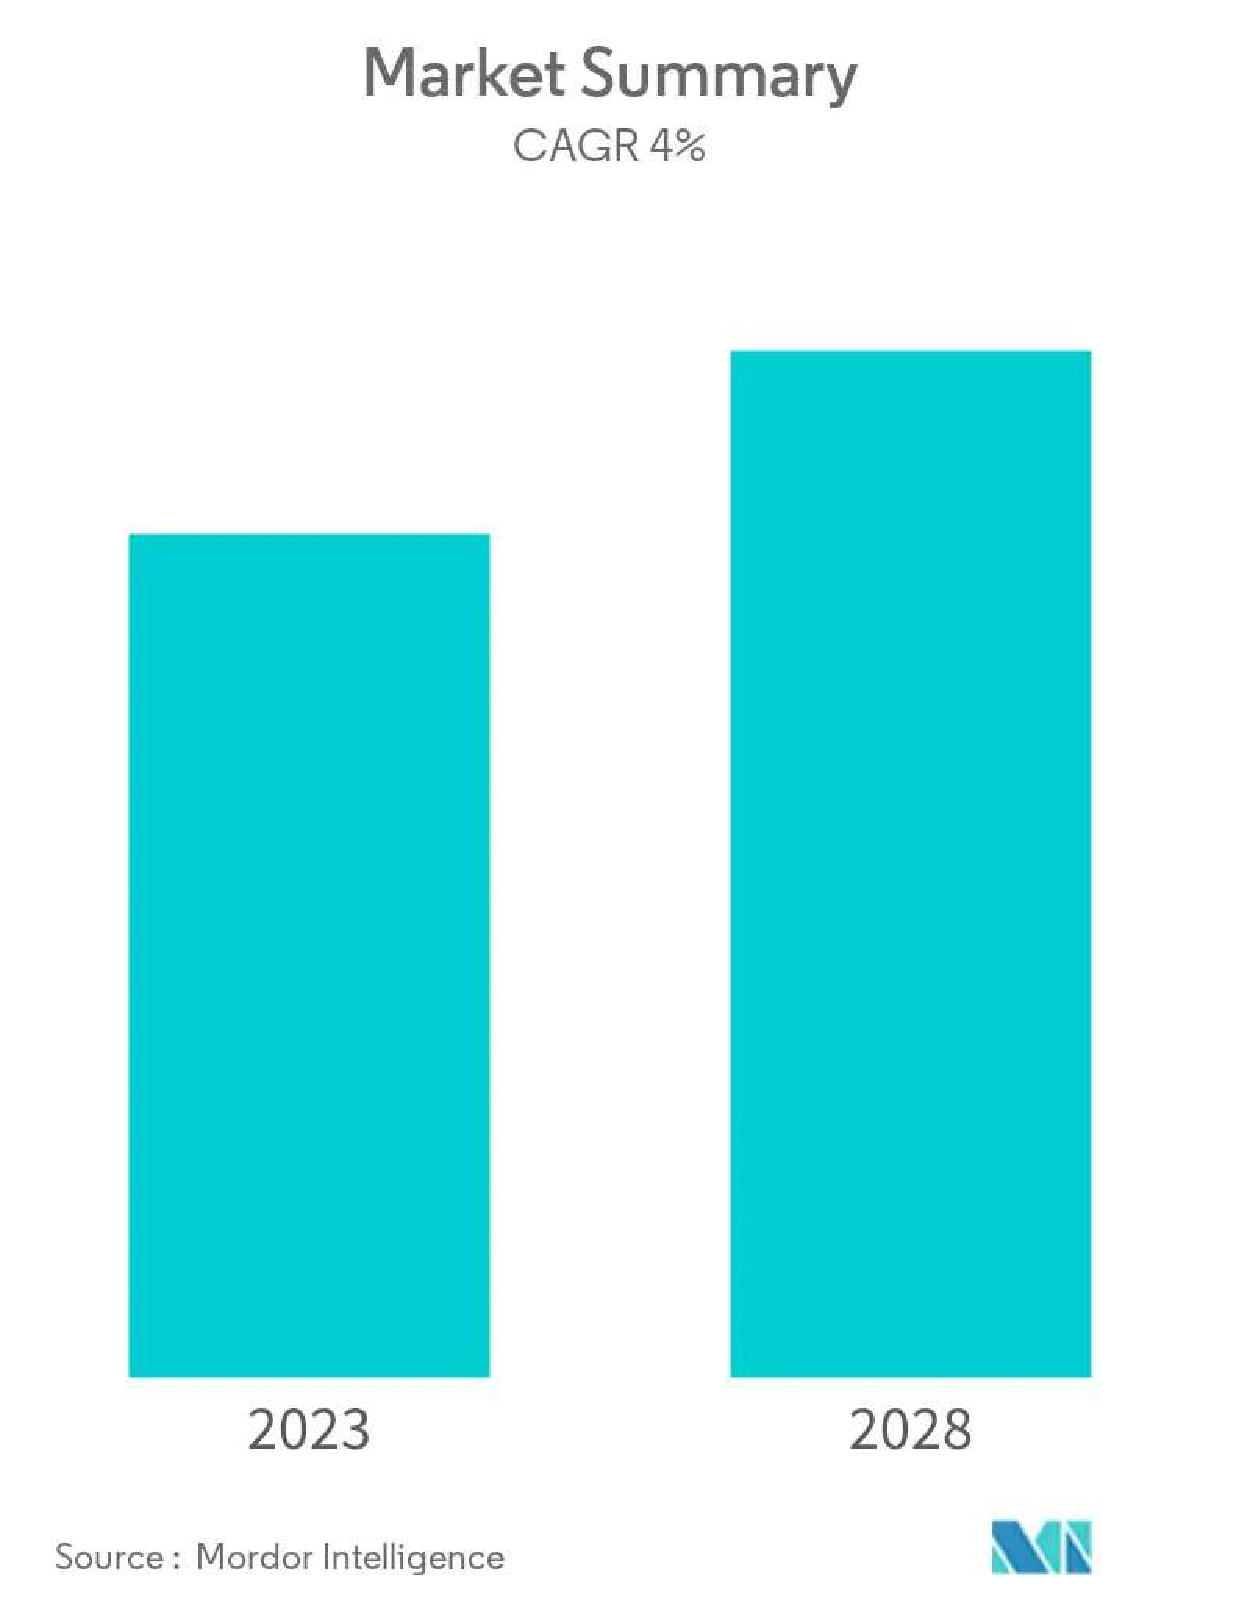
\includegraphics[width=\columnwidth/3]{images/smartphones-market_Market_Summary.pdf}
  \caption{Mercado de Smartphones - crescimento, tendências, impacto da COVID-19 e previsões (2023 - 2028).}
  \acsfont{Fonte: \cite{intelligence_2023}}
  \label{fig:smartphones-market_Market_Summary}
\end{figure}

Para situar onde os \acp{dm} chegaram, é preciso olhar um pouco o passado para lembrar como os computadores eram: máquinas que ocupavam salas gigantes, os quais eram manuseados somente por setores importantes da sociedade, antes mesmo de ser um dispositivo doméstico como é hoje, limitando-se a órgãos do governo, instituições de ensino e poucas empresas, por exemplo \citet{alecrim_2013}.

Com o desenvolvimento da tecnologia, os computadores tornaram-se cada vez mais compactos, eficientes, práticos e fáceis de usar, podendo ser levados para qualquer lugar, por qualquer pessoa. As tecnologias que fornecem essa maior flexibilidade são conhecidas como \acp{dm}.

Sintetizando, um \ac{dm} é um tipo de dispositivo computacional que tem como principais características a portabilidade, a compactabilidade e fácil manuseio \citet{lee2005aplicaccoes}, além de todos os aspectos citados na seção \ref{sec:mobilidade}. 

De acordo com \citet{laricchia_2022}, em 2021, o número de \acp{dm} operando em todo o mundo ficou em quase 15 bilhões, contra pouco mais de 14 bilhões no ano anterior. Espera-se que o número de \acp{dm} atinja 18,22 bilhões até 2025, um aumento de 4,2 bilhões de dispositivos (aproximadamente 30\%) em comparação com os níveis de 2020. A \figref{fig:mobiles20to25} mostra o gráfico desta previsão.

\begin{figure}[H]
\centering
  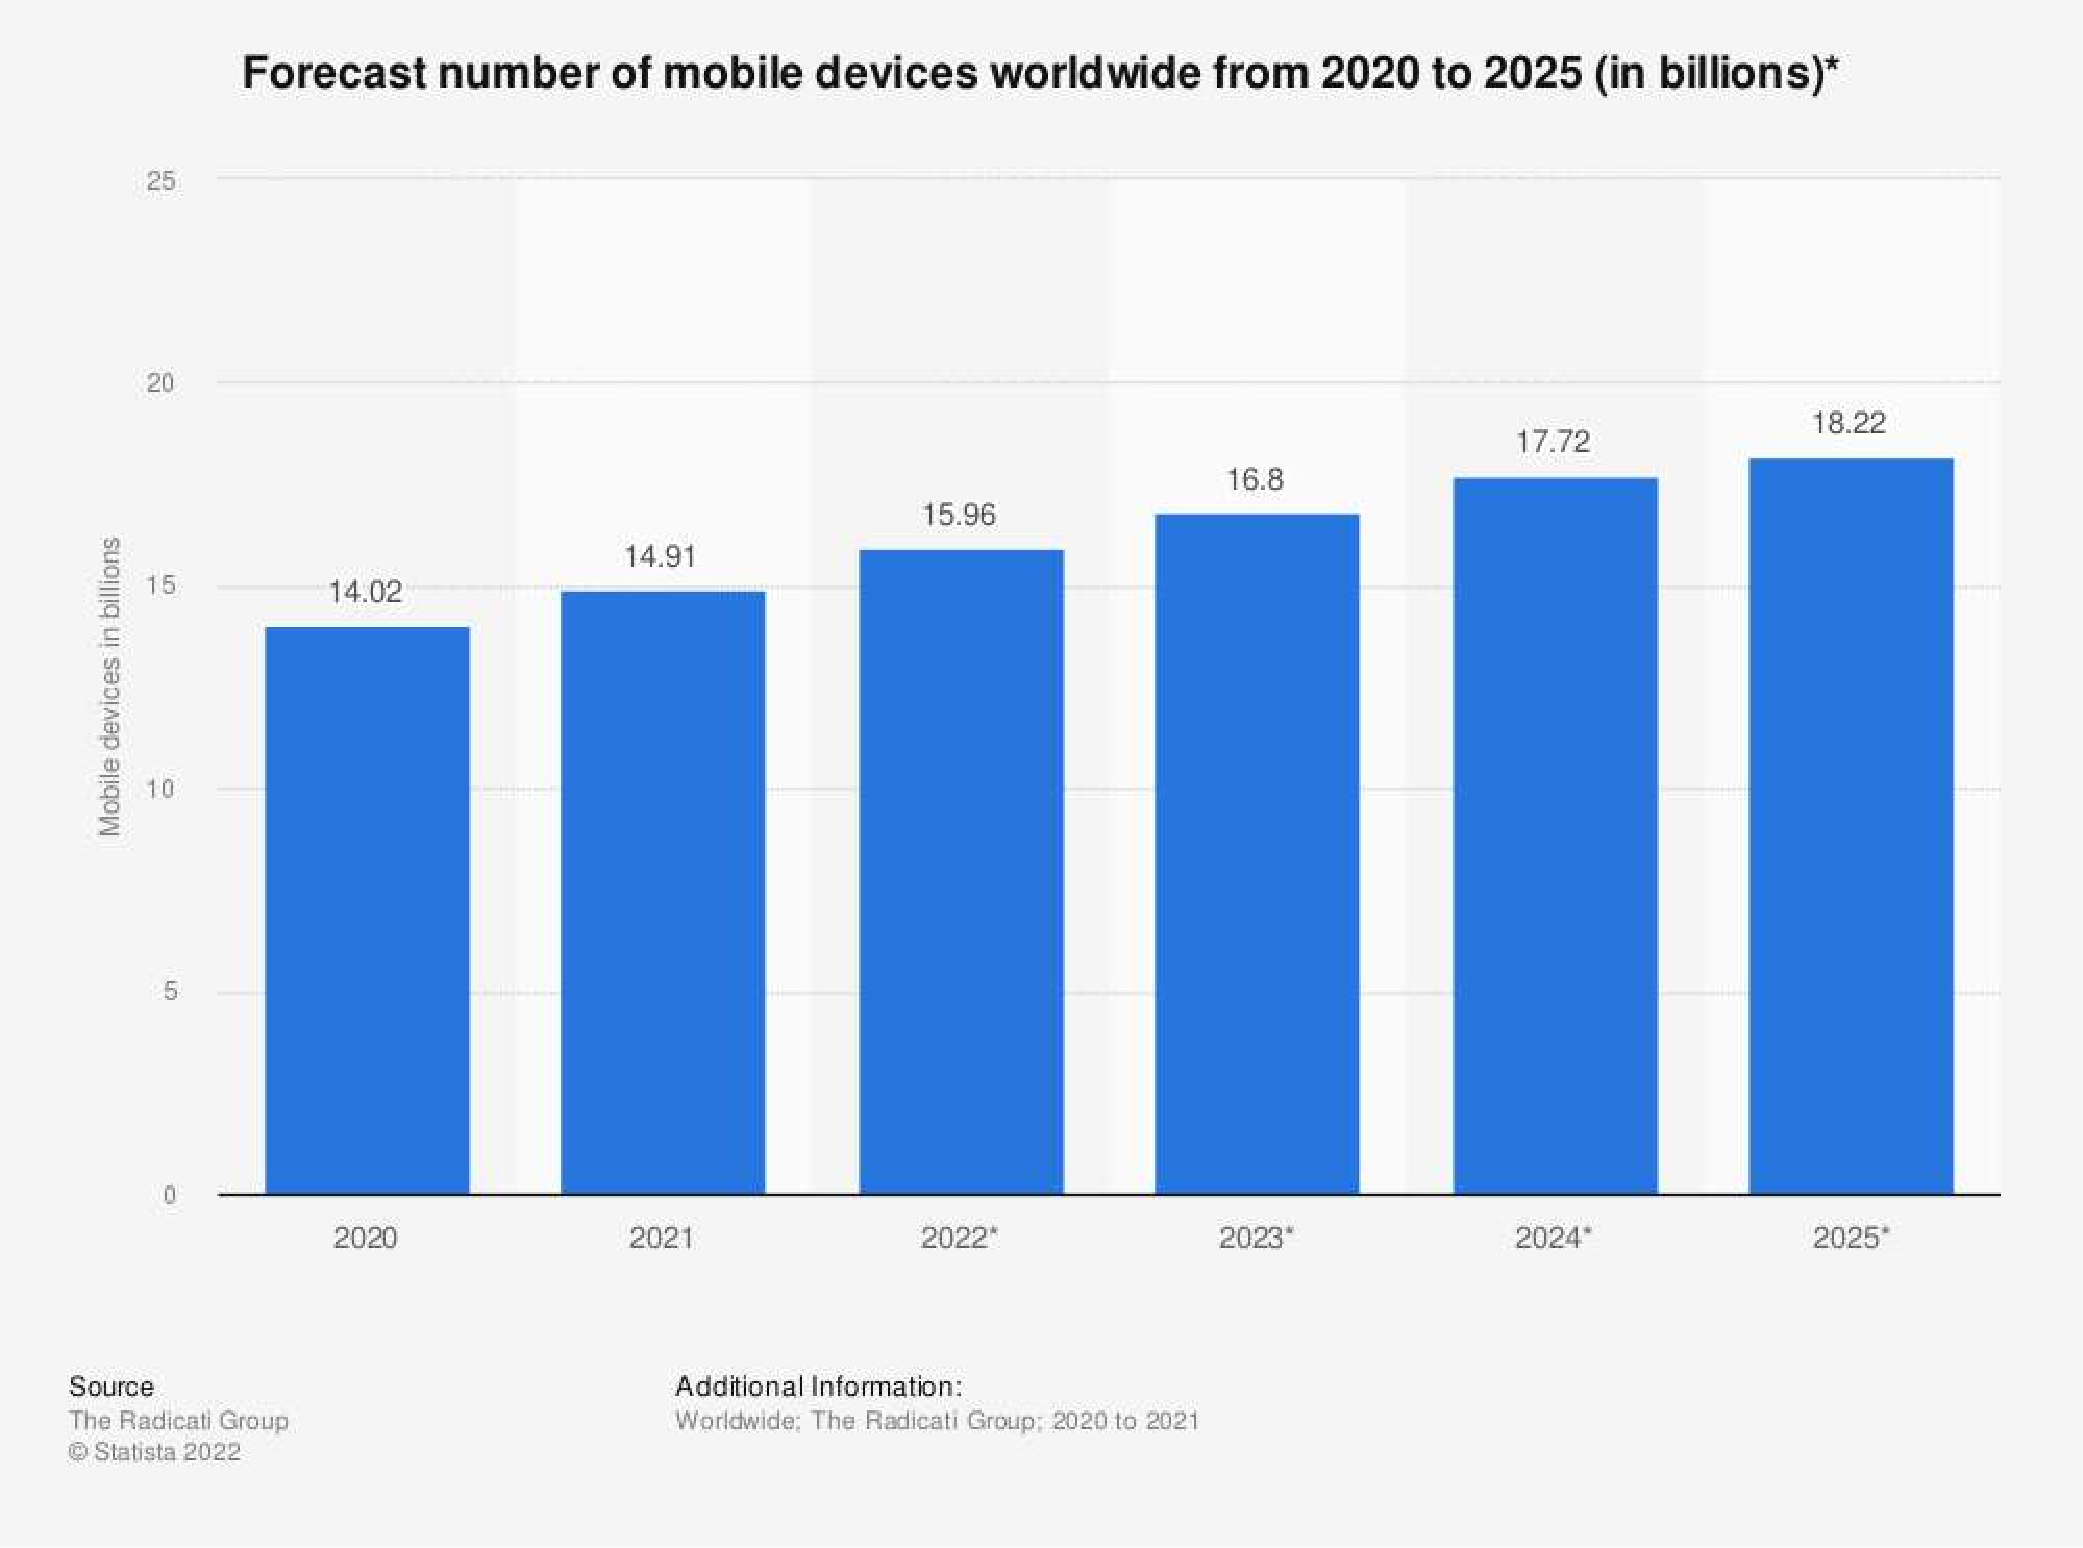
\includegraphics[scale=0.35]{images/mobiles20to25.pdf}
  \caption{Previsão do número de dispositivos móveis em todo o mundo de 2020 a 2025 (em bilhões).}
  \acsfont{Fonte: \citet{laricchia_2022}}
  \label{fig:mobiles20to25}
\end{figure}

Visto esse crescimento no uso de \acp{dm}, é perceptível que a demanda por \textbf{desenvolvimento de \textit{software}} para esta tecnologia também aumentou. Essas soluções são chamadas de aplicativos móveis, tema que será abordado com mais detalhes na seção \ref{sec:apps} e posteriormente detalhado sobre o mercado de desenvolvimento de \acp{app} na subseção \ref{ssec:dev_apps}.

Falar sobre \acp{dm} é falar também de sobre seus \acp{so}, pois estes são responsáveis por gerenciar e controlar o \textit{hardware}  e \textit{software} dos mesmos, atualmente, os principais são o iOS da Apple e o Android da Google. Ambos \acp{so} tem características específicas e oferecem diferentes níveis de personalização e integração com outros dispositivos e serviços.

Desta forma, a existência destes dois grandes \acp{so} de \acp{dm} é devido à competição entre as empresas de tecnologia para oferecer a melhor experiência do usuário e atrair o maior número de usuários para seus dispositivos. Além disso, os \acp{so} também são importantes para garantir a compatibilidade com \acp{app} e jogos, bem como para garantir a segurança e privacidade dos dados do usuário. Eles também possibilitam acesso a recursos como câmera, GPS, conectividade com a internet e outros dispositivos, além de gerenciar a bateria e os recursos de armazenamento; as peculiaridades e mercado de ambos \acp{so} serão abordados brevemente a seguir, em suas respectivas subseções.

\subsection{iOS}\label{ssec:ios}
O iOS é o \ac{so} móvel desenvolvido pela Apple e utilizado em dispositivos como iPhones, iPads e iPods Touch. O iOS tem se tornado cada vez mais popular desde o seu lançamento em 2007, desde então tem sido atualizado regularmente com novas funcionalidades e melhorias de desempenho, ele é considerado por muitos acadêmicos como um dos \acp{so} móveis mais avançados do mercado.

De acordo com \citet{borges2017analise}, o iOS é considerado mais fácil de usar e mais seguro que o Android. Os usuários também relataram uma melhor experiência de usuário com o iOS, incluindo uma interface mais limpa e intuitiva. Isso se deve principalmente ao fato de que o iOS é um sistema fechado, feito para \textit{hardwares} próprios e com um controle de qualidade e desempenho arrojado, visto que os dispositivos que rodam o sistema são produzidos pela mesma empresa que desenvolve seu \textit{software}, fazendo então com que hajam menos falhas causadas por incompatibilidades ou quebra de diretrizes, como pode acontecer em outros \acp{so} que são livres para utilização em diversos dispositivos.

A segurança também é uma preocupação importante para o iOS, visto que o \ac{so} inclui várias medidas de segurança para proteger os dados do usuário, como a autenticação biométrica de toque ou rosto, criptografia de dados, configurações rígidas de privacidade e \acp{app} de segurança integrados. Além disso, o iOS recebe atualizações regulares para corrigir vulnerabilidades de segurança e adicionar novos recursos de segurança. \cite{ahvanooey2020survey}. 

Segundo \cite{stats2020mobile}, como mostrado nos gráficos das \figref{fig:mobile_operating_system_market_share_w} e \figref{fig:mobile_operating_system_market_share_br} em destaque logo abaixo, o iOS tem um mercado geral que corresponde a cerca de \nicefrac{1}{3} do mercado que tem o Android, no Brasil, no último ano, esse percentual aumentou, seguindo a tendência do resto do mundo. Muitas coisas influenciam essa diferença de mercado, mas o maior ponto é o preço, visto que para ter os dispositivos da Apple requer um investimento bem maior que um Android, que possui uma grande variedade de dispositivos e portanto preços, essa diferença pode aumentar ainda mais de acordo com a economia do país em questão, como o caso do Brasil, por exemplo.

\begin{figure}[H]
\centering
\begin{subfigure}{\textwidth}
   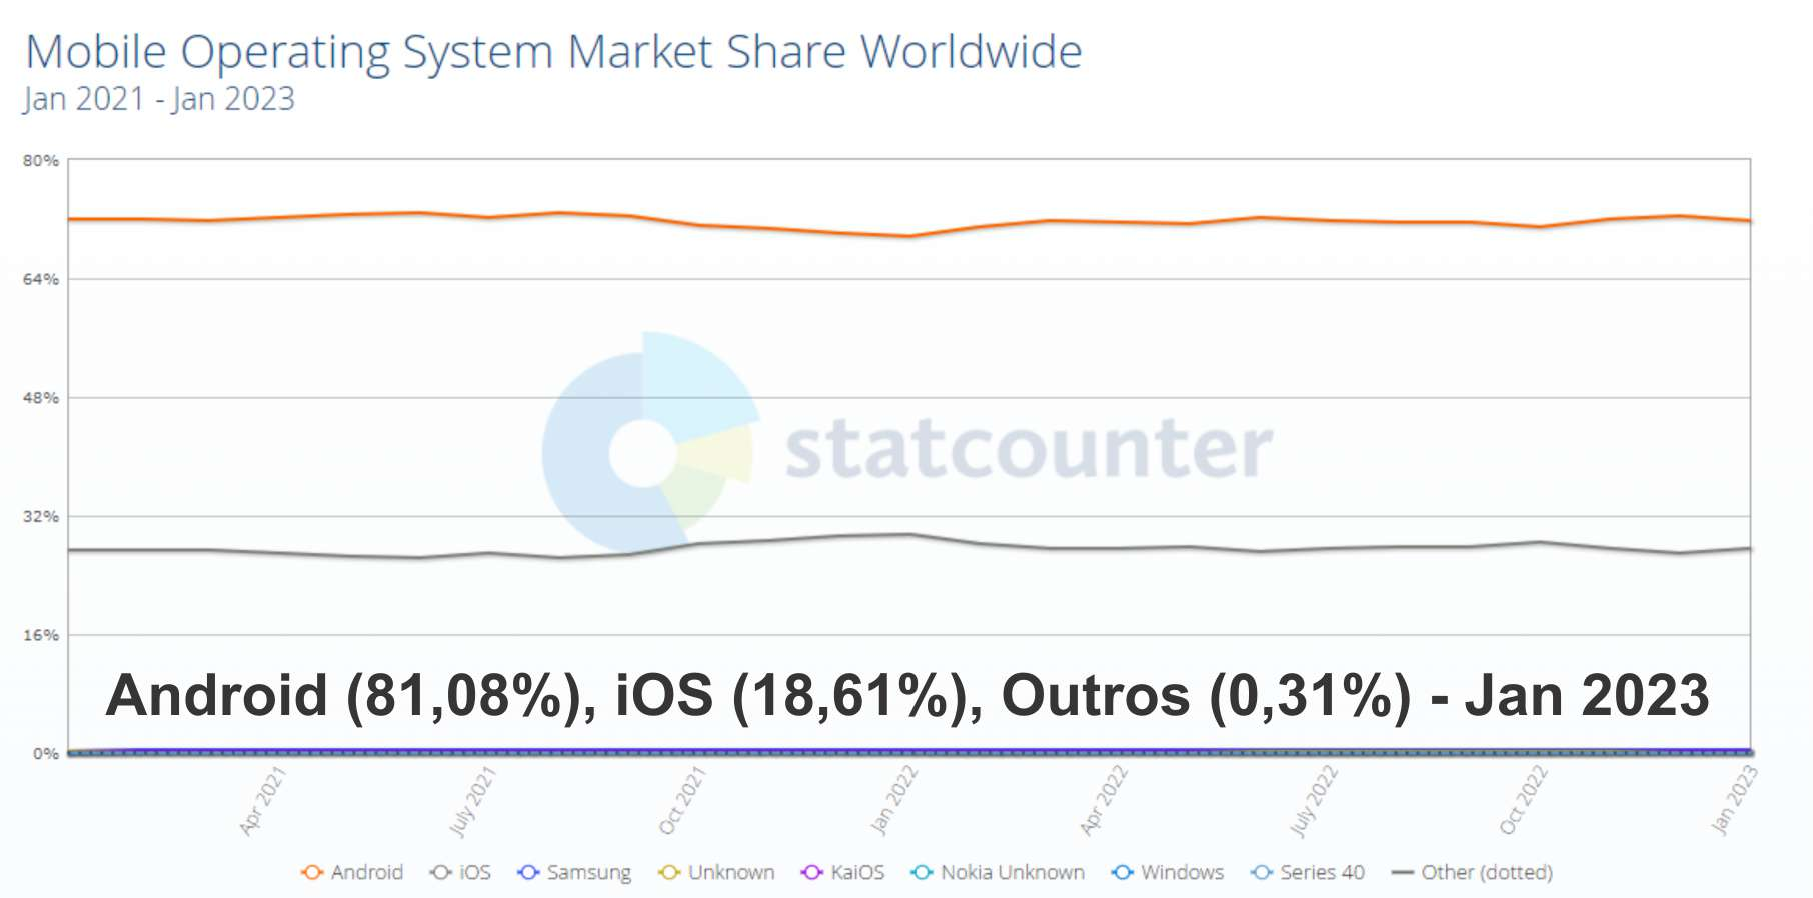
\includegraphics[width=1\linewidth]{images/mobile_operating_system_market_share_w.pdf}
   \caption{Participação no mercado de Sistemas Operacionais móveis em todo o mundo.}
   \acsfont{Fonte: \cite{stats2020mobile}}
   \label{fig:mobile_operating_system_market_share_w} 
\end{subfigure}

\begin{subfigure}{\textwidth}
   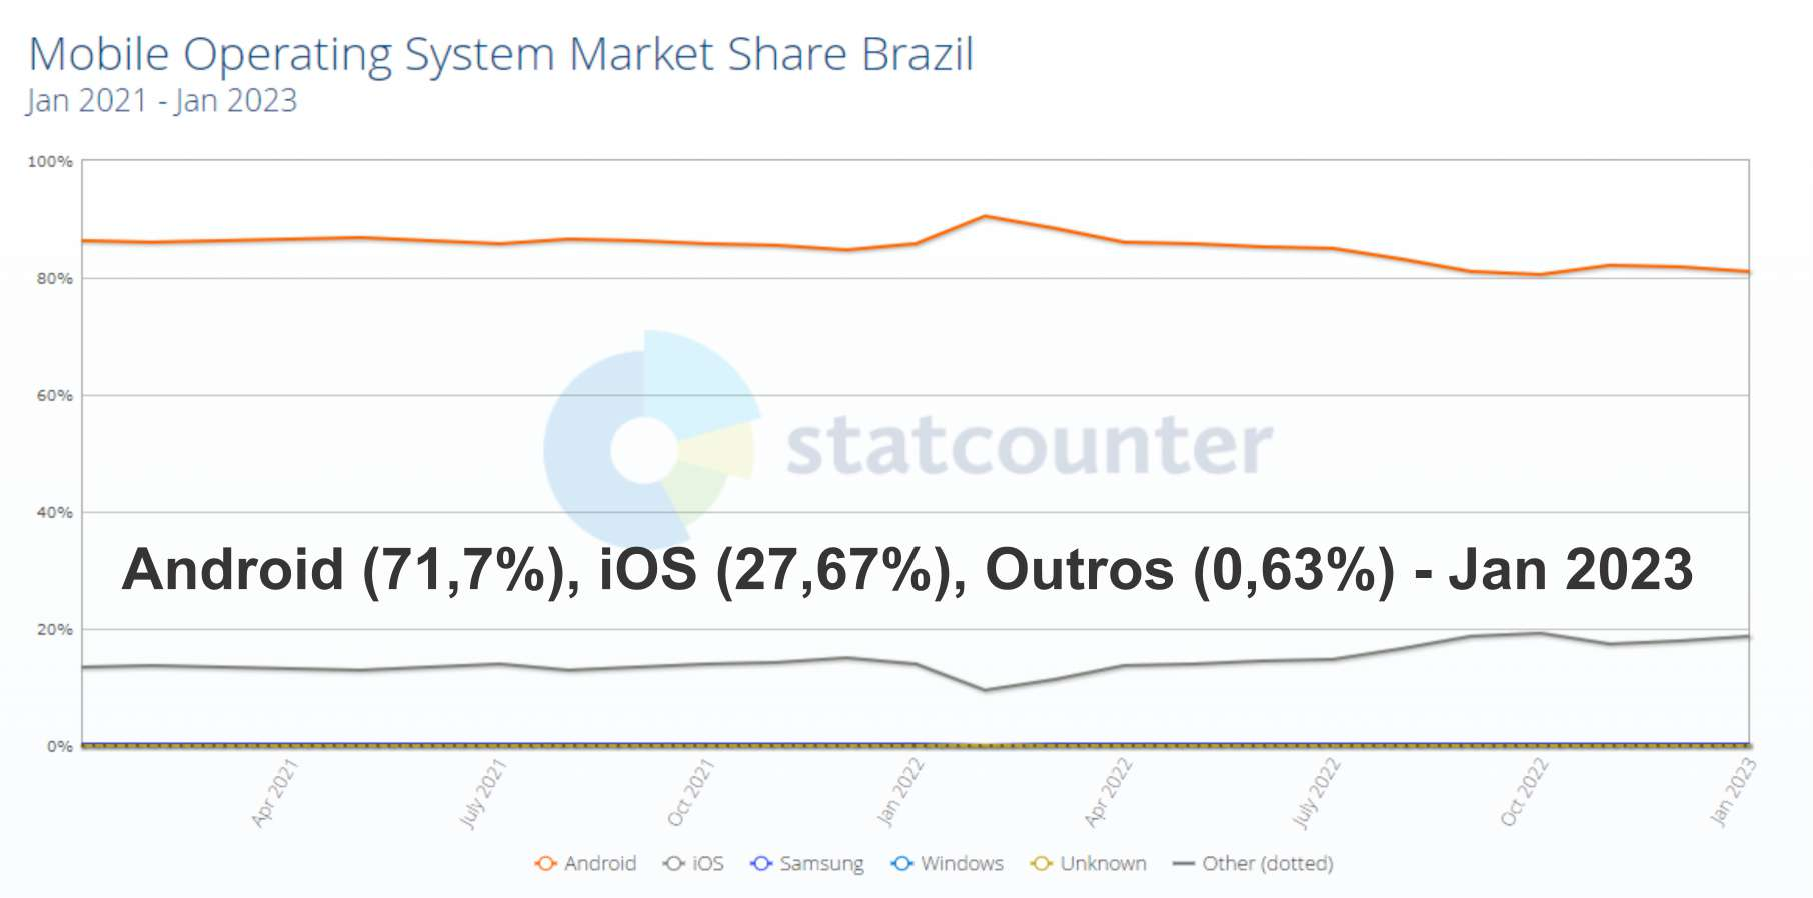
\includegraphics[width=1\linewidth]{images/mobile_operating_system_market_share_br.pdf}
   \caption{Participação no mercado de Sistemas Operacionais móveis no Brasil.}
   \acsfont{Fonte: \cite{stats2020mobile}}
   \label{fig:mobile_operating_system_market_share_br}
\end{subfigure}
\end{figure}

% \begin{figure}[h]
% \centering
% \subfigure[Participação no mercado de Sistemas Operacionais móveis em todo o mundo]{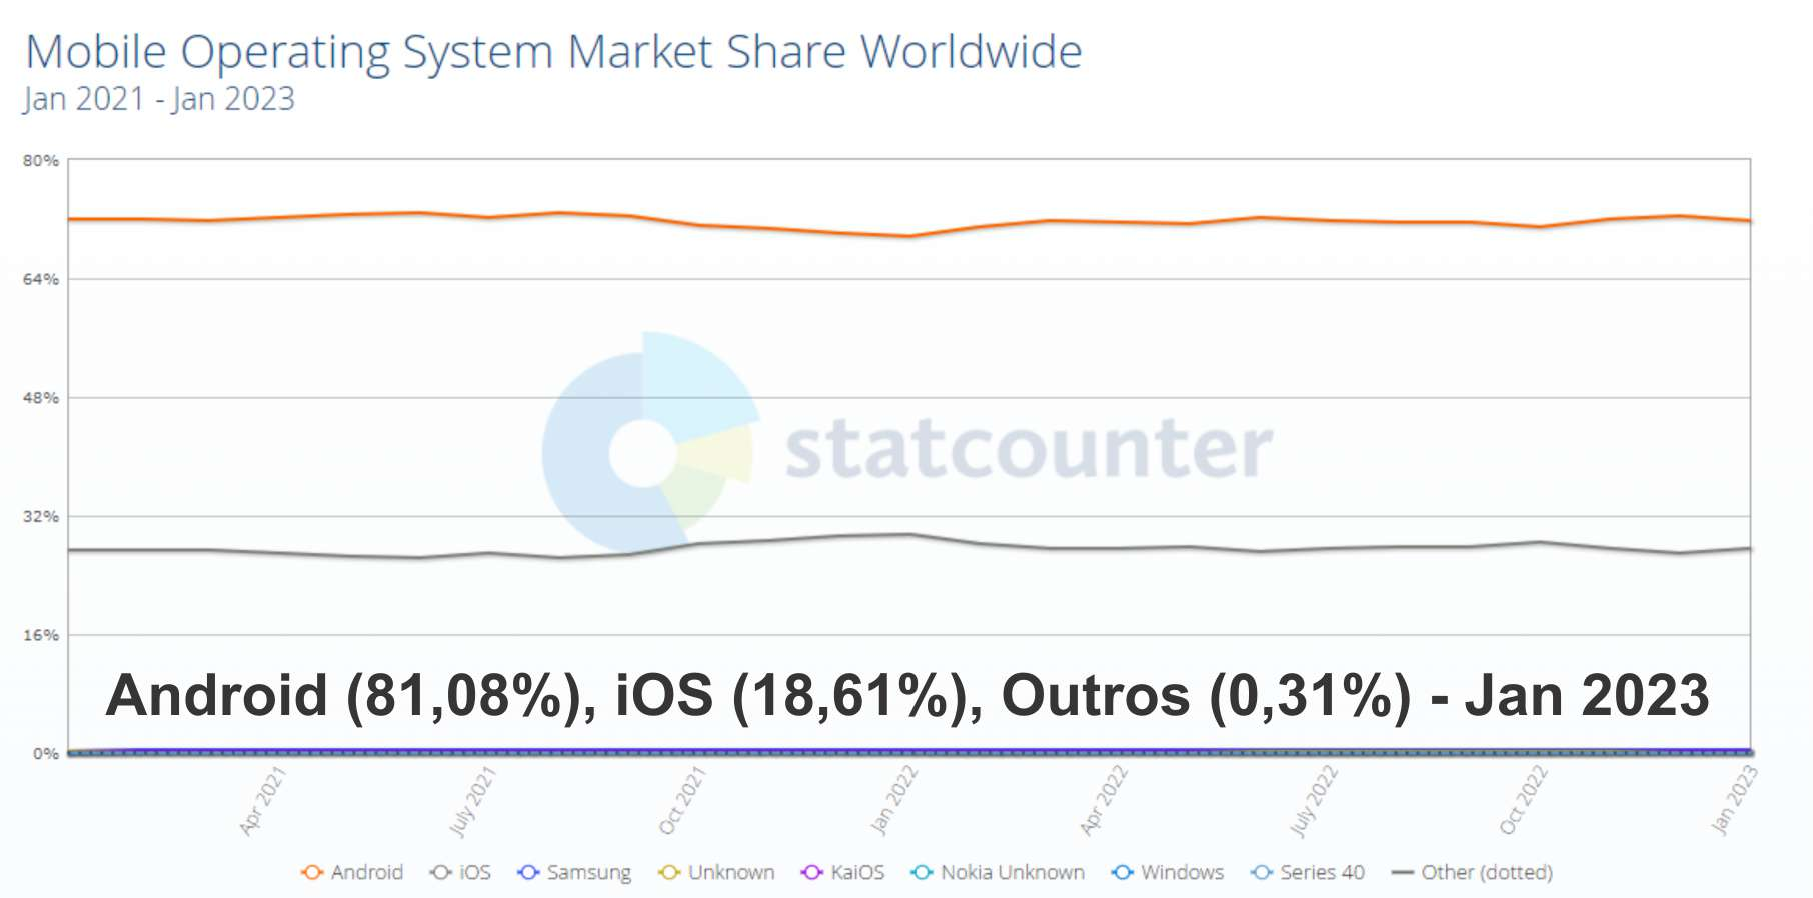
\includegraphics[width=0.47\linewidth]{images/mobile_operating_system_market_share_w.pdf}\label{fig:mobile_operating_system_market_share_w}}
% \qquad
% \subfigure[Participação no mercado de Sistemas Operacionais móveis no Brasil]{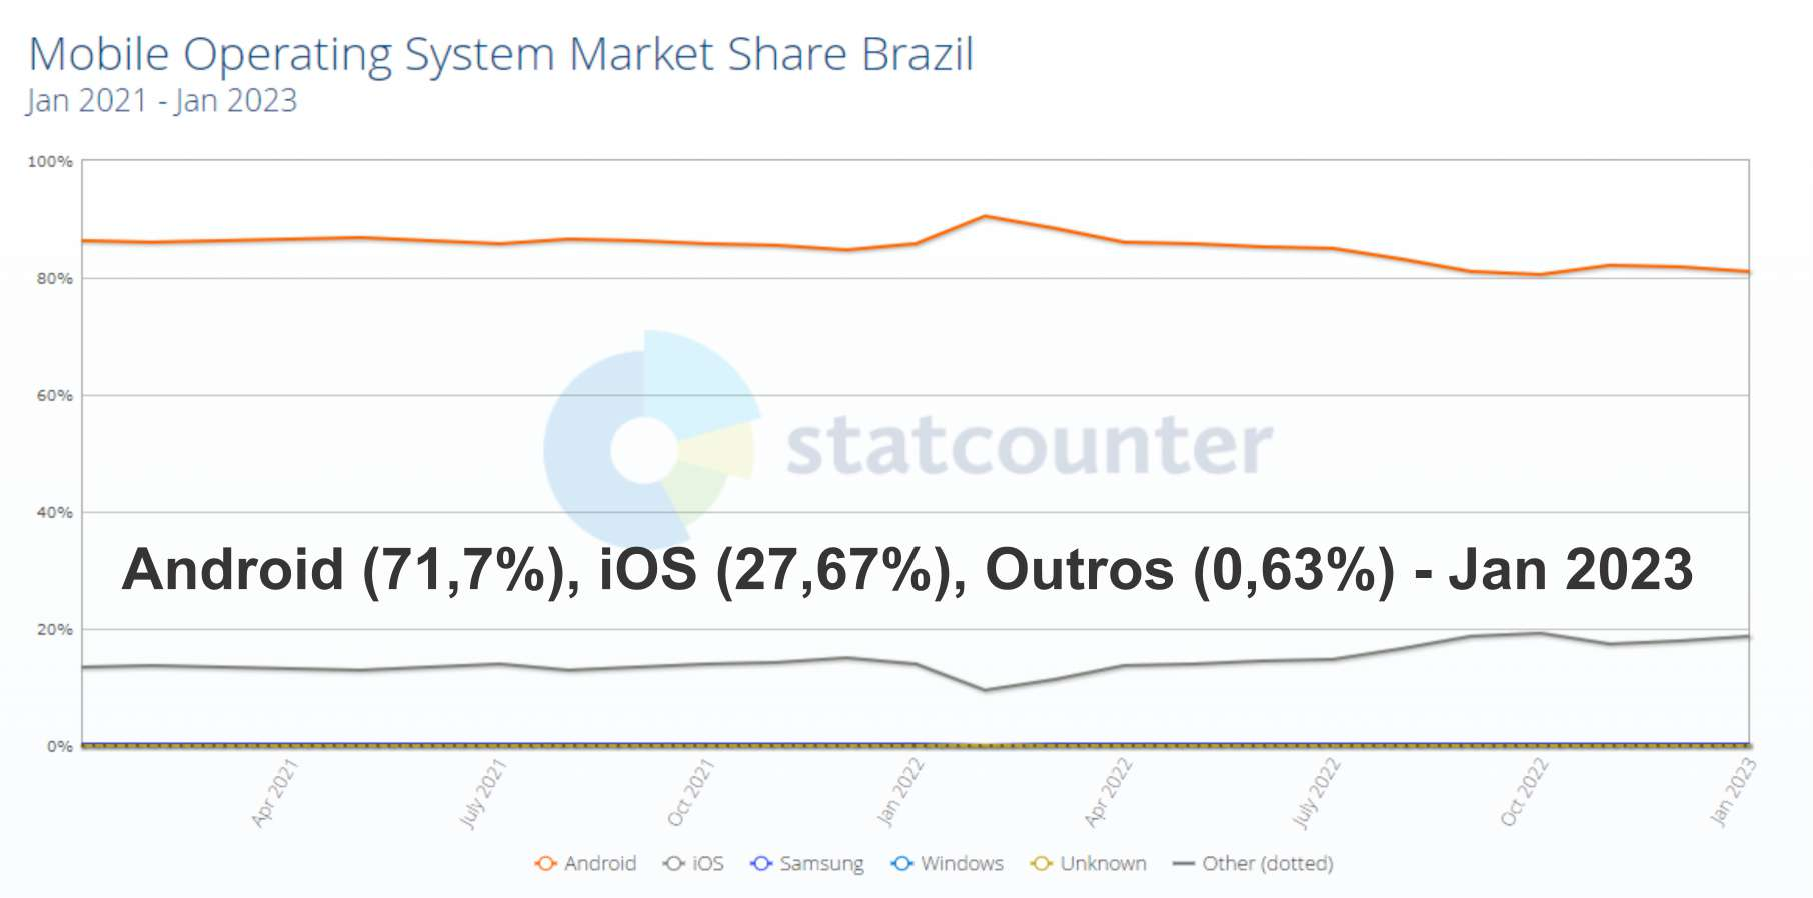
\includegraphics[width=0.47\linewidth]{images/mobile_operating_system_market_share_br.pdf}\label{fig:mobile_operating_system_market_share_br}}
% \qquad
% \caption[Participação no mercado de Sistemas Operacionais móveis, dados do Brasil e do mundo]{(a) Participação em todo o mundo (b) Participação no Brasil}
% \end{figure}

%--------------------------------------------------------------------
\subsection{Android}\label{ssec:android}
O \ac{so} Android é desenvolvido pela Google e é usado em \acp{dm}, como smartphones e tablets. Ele foi lançado em 2008 e tem sido atualizado regularmente com novas funcionalidades e melhorias de desempenho.

De acordo com a pesquisa "Comparativo entre Sistemas Operacionais móveis - Android x iOS" \citet{leite2017comparativo}, o Android tem uma maior flexibilidade e personalização do que o iOS, permitindo que os usuários ajustem a interface de acordo com suas necessidades. Além disso, os dispositivos Android também tendem a ter uma melhor relação custo-benefício do que os dispositivos iOS.

Embora o Android tenha alguns problemas de segurança adicionais devido à sua abertura e personalização, a Google tem trabalhado para melhorar a confiabilidade do \ac{so}, incluindo a implementação de medidas de proteção como a verificação de segurança do Google Play Protect.

Em resumo, o \ac{so} Android é considerado flexível, personalizável e com uma boa relação custo-benefício, além de ser uma opção segura e com ampla variedade de \acp{app} disponíveis na Google Play Store, ofertando um leque de \acp{app} comparável à da App Store da Apple, o que a torna uma escolha atraente para muitos usuários. As pesquisas mencionadas acima (\citet{leite2017comparativo} e \citet{borges2017analise}) apoiam essa avaliação.

Assim como para o iOS, pode-se olhar os números de dispositivos Android no Brasil e no mundo, segundo os mesmos dados de \cite{stats2020mobile}, mostrado nos gráficos das \figref{fig:mobile_operating_system_market_share_w} e \figref{fig:mobile_operating_system_market_share_br} acima, o Android domina com grande folga em ambos os cenários, muito influenciado pelo preço e amadurecimento em relação às diversas funcionalidades agregadas ao \ac{so}.

\section{Aplicativos móveis}\label{sec:apps}
É indiscutível que os aplicativos móveis tornaram-se uma parte fundamental da vida cotidiana das pessoas, permitindo que elas realizem uma generosa quantidade de tarefas em seus \acp{dm}. Com o crescimento contínuo do mercado de aplicativos móveis, o desenvolvimento de aplicativos móveis se tornou uma área em rápida expansão para empresas e desenvolvedores.

Nesta seção, serão tratadas algumas informações gerais sobre o desenvolvimento de \acp{app} e uma visão sobre o desenvolvimento híbrido \textit{versus} desenvolvimento nativo.

\subsection{Desenvolvimento de aplicativos}\label{ssec:dev_apps}
O desenvolvimento de aplicativos, ou desenvolvimento de \textit{software} para dispositivos móveis, é um campo em constante evolução, com novas tecnologias e abordagens surgindo a cada dia.

Segundo \cite{Marconi2021}, o desenvolvimento de aplicativos móveis requer um conjunto de habilidades técnicas e conhecimentos específicos em design de interface do usuário, programação e arquitetura de \textit{software}. Além disso, é importante considerar as di\-fe\-ren\-tes plataformas móveis, como as já citadas \nameref{ssec:ios} e \nameref{ssec:android}, e suas respectivas diretrizes de desenvolvimento.

Existem diversas ferramentas e \textit{frameworks} disponíveis para facilitar o processo de desenvolvimento, como o Android Studio para desenvolvimento de \acp{app} Android com \textit{Java} ou \textit{Kotlin}, o Xcode para iOS, usando \textit{Swift} ou \textit{Objective-C}, ou o VSCode — um editor de código-fonte gratuito e de código aberto desenvolvido pela Microsoft — usado também para as alternativas anteriores, mas principalmente para o desenvolvimento multiplataforma com React Native ou Flutter, que vem ganhando popularidade por sua rapidez e facilidade de uso.

Um dos principais desafios no desenvolvimento de aplicativos móveis é a garantia de que o \ac{app} funcione corretamente em diferentes dispositivos e tamanhos de tela. Para isso, é fundamental realizar testes e validações em várias plataformas e dispositivos, a fim de garantir a qualidade do \textit{software} desenvolvido \cite{Biswal2020}.

\subsubsection{Desenvolvimento nativo}\label{sssec:dev_apps_nativo}
O desenvolvimento de \textit{software} nativo para \acp{dm} consiste em criar \acp{app} específicos para um determinado \ac{so}, utilizando as linguagens de programação e ferramentas oferecidas por esses sistemas, como os já citados Android com \textit{Java} ou \textit{Kotlin} e o iOS com \textit{Swift} ou \textit{Objective-C}. Essa abordagem permite que o \ac{app} seja otimizado para o \ac{so} em questão, garantindo maior desempenho e uma melhor experiência para o usuário final.

Segundo uma revisão sistemática realizada por \cite{Sarker2021}, o desenvolvimento nativo tem sido a escolha mais comum para desenvolvedores de aplicativos móveis, principalmente devido à sua eficiência e desempenho. Além disso, o desenvolvimento nativo permite o acesso completo às APIs e recursos do sistema operacional, o que possibilita a criação de \acp{app} mais avançados e sofisticados.

No entanto, o desenvolvimento nativo também pode ser mais trabalhoso e exigir um conhecimento mais aprofundado das tecnologias envolvidas. De acordo com \cite{Biswal2020}, a complexidade do processo de desenvolvimento nativo pode ser amenizada pelo uso de ferramentas e \textit{frameworks} especializados, como o Android Studio e o Xcode.

\subsubsection{Desenvolvimento híbrido}\label{sssec:dev_apps_hibrido}
O desenvolvimento de \textit{software} híbrido para \acp{dm} pode ser realizado utilizando diversas tecnologias e \textit{frameworks}, como as duas que estão em alta atualmente: Flutter e React Native. Em resumo, ambos são \textit{frameworks} que permitem criar \acp{app} nativos para Android e iOS a partir de um único código-base, claro que com algumas diferenças entre si, como o desempenho, linguagem, método de criação de componentes, etc.

Uma comparação entre as duas tecnologias foi realizada por \cite{GuhaBanerjee2020}, que avaliaram a performance e a experiência do usuário em diferentes cenários. Os resultados indicaram que o Flutter apresentou uma performance superior em termos de tempo de carregamento e suavidade de animações, enquanto o React Native foi mais eficiente em termos de uso de memória e processamento. Além disso, ambos os \textit{frameworks} ofereceram uma ex\-pe\-ri\-ên\-ci\-a de usuário semelhante ao desenvolvimento nativo, com recursos como acesso a câmera, geolocalização e notificações \textit{push}.

\begin{figure}[H]
\centering
  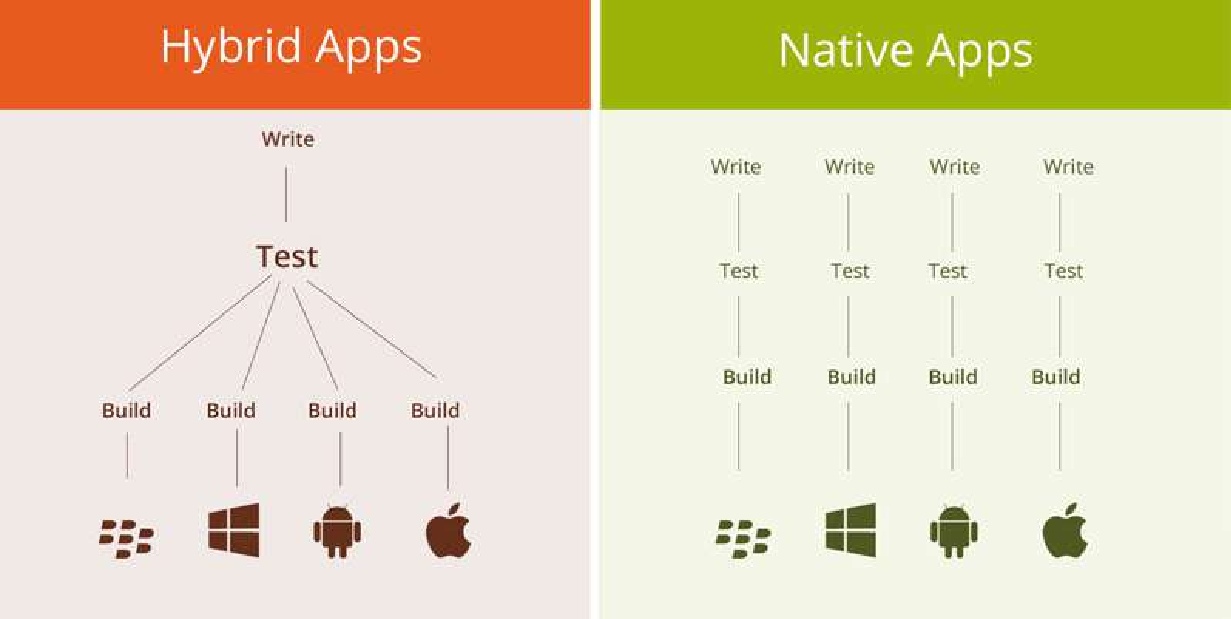
\includegraphics[width=\columnwidth]{images/native-diff.pdf}
  \caption{Passos do desenvolvimento de \acp{app} híbridos e nativos.}
  \acsfont{Fonte: \cite{AngularMinds}}
  \label{fig:native_diff}
\end{figure}

A imagem acima mostra a diferença do desenvolvimento de um \ac{app} híbrido (multiplataforma) para um \ac{app} nativo, pode-se notar que o desenvolvimento híbrido economiza tempo, esforço e consequentemente dinheiro, por reduzir etapas, tornando-se uma escolha altamente viável e amplamente utilizada atualmente.

Portanto, a escolha entre as duas tecnologias pode depender de diferentes fatores, como a preferência da equipe de desenvolvimento, a complexidade do \ac{app} e a disponibilidade de recursos e ferramentas. É importante avaliar as características e limitações de cada tecnologia antes de decidir qual utilizar em um projeto. Neste projeto em particular — para o desenvolvimento do \ac{app} — a escolha foi o Flutter, o qual será destrinchado a seguir na seção \ref{sec:flutter}.

\section{APIs \textit{Web}}\label{sec:apis_web}
\ac{api}, que em português significa "Interface de Programação de Aplicativos", é um conjunto de rotinas e padrões de programação que permitem a integração de diferentes sistemas ou plataformas. É através de uma \ac{api} que é possível fazer a comunicação entre duas aplicações, permitindo que uma delas utilize os serviços ou dados oferecidos pela outra. As \acp{api} são geralmente disponibilizadas por empresas ou organizações para que desenvolvedores possam criar novas aplicações ou integrar funcionalidades em sistemas existentes. Esse tipo de aplicação utiliza a internet para a transferência
de dados e processa e armazena informações relevantes para o funcionamento de um produto
ou serviço.

Segundo \cite{martin2008codigolimpo}, as \acp{api} podem ser classificadas em duas categorias principais: as \textit{Web} \acp{api} e as \acp{api} de \textit{software}. As \textit{Web} \acp{api} são acessadas através da internet utilizando protocolos como \ac{http} e geralmente são disponibilizadas por meio de \acp{url} específicas — que em tradução livre significa "Localizador Uniforme de Recursos", ou seja, o endereço web, o texto digitado na barra do navegador para acessar uma determinada página ou serviço — que retornam dados em formatos padronizados como \ac{json} ou \ac{xml}, geralmente usando o padrão \ac{rest}, um estilo arquitetural que define como sistemas distribuídos devem se comunicar. Já as \acp{api} de \textit{software} são usadas para acessar serviços em nível de \ac{so} ou \textit{software} e geralmente são escritas em linguagens de programação específicas.

\begin{figure}[H]
\centering
  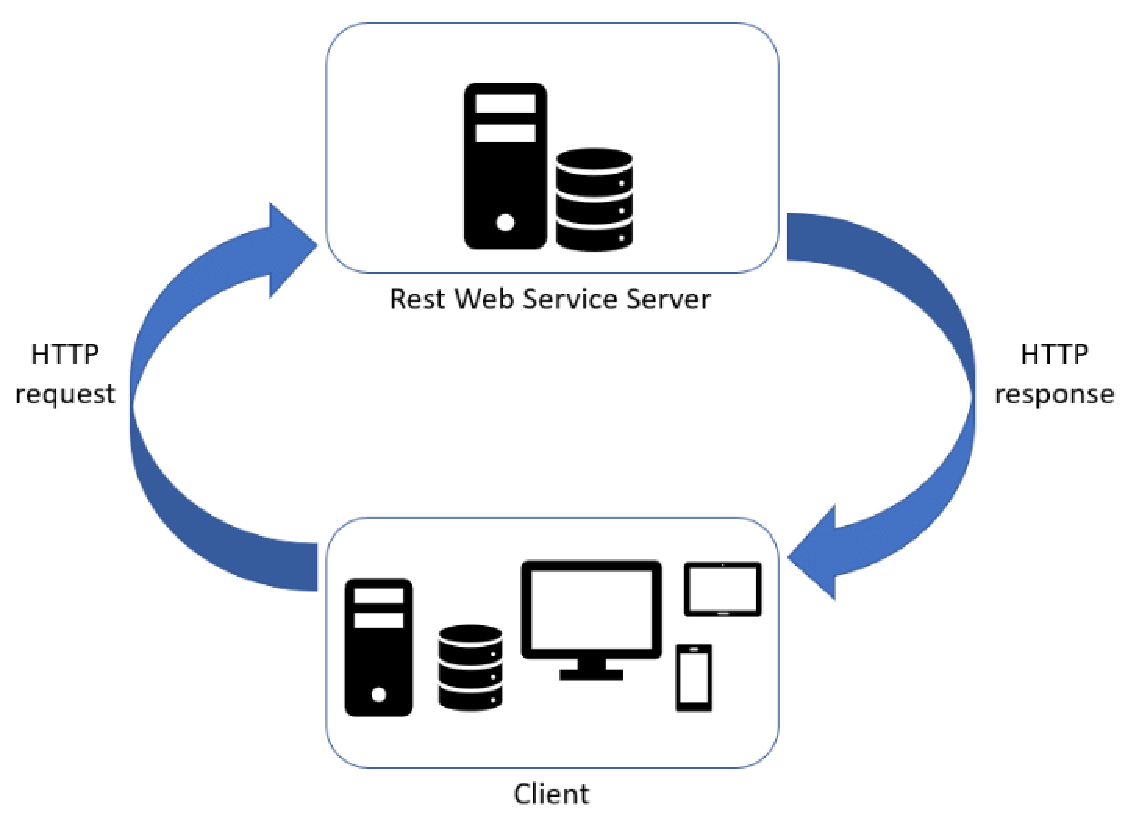
\includegraphics[width=\columnwidth]{images/REST-API-synchronous-communication-schema.pdf}
  \caption{Esquema de comunicação síncrona da \ac{api} \ac{rest}.}
  \acsfont{Fonte: \cite{Bertoli2021}}
  \label{fig:REST-API}
\end{figure}

Uma \ac{api} funciona baseado na conversação entre cliente e servidor, através de um protocolo de comunicação, que fica responsável por transpor os dados entre um e outro, este processo envolve três passos, o primeiro é a geração de uma solicitação pelo cliente ao servidor, geralmente através do protocolo \ac{http}. Em seguida, se a solicitação exigir acesso ao banco de dados, o servidor realizará a consulta necessária para obter as informações solicitadas. Por fim, após obter a resposta, o servidor a encaminha para o cliente.


\section{Flutter}\label{sec:flutter}
O Flutter, principal tecnologia aplicada no desenvolvimento deste \ac{app}, é um framework de desenvolvimento de aplicativos móveis, desenvolvido pela Google, criado em 2014 (originalmente chamado de \textit{Sky}), mas que só veio disputar como solução para desenvolvimento multiplataforma em 2018 quando teve sua primeira versão estável lançada, o Flutter permite criar \acp{app} nativos para Android e iOS a partir de um único código-base. Ele utiliza a linguagem de programação \textit{Dart} — também criada pelo Google — que é uma linguagem moderna e orientada a objetos, com recursos avançados como \textit{garbage collection}, tipagem forte e \textit{async/await}.

O Flutter tem ganhado popularidade entre os desenvolvedores devido à sua produtividade e flexibilidade, além de oferecer uma experiência de usuário fluida e rica em animações. Ele também possui um rico conjunto de \textit{widgets} e bibliotecas que tornam a criação de interfaces de usuário complexas mais simples e intuitivas.

Uma avaliação do Flutter em relação a outras tecnologias de desenvolvimento de aplicativos móveis foi realizada por \cite{Zhou2021}, que analisaram a usabilidade, desempenho e eficiência do Flutter em comparação com o React Native e o desenvolvimento nativo. Os resultados indicaram que o Flutter ofereceu uma experiência de usuário superior em relação ao React Native e uma performance comparável ao desenvolvimento nativo, além de apresentar uma curva de aprendizado mais suave e uma maior eficiência no desenvolvimento de protótipos. Estes pontos reforçam a escolha do Flutter como principal \textit{framework} escolhido para o projeto.

Dados de interesse do Google\footnote{\label{google_trends_flutter_react}Google Trends: \url{https://trends.google.com/trends/explore?date=2018-01-02\%202023-01-03&q=\%2Fg\%2F11h03gfxy9,\%2Fg\%2F11f03_rzbg}} corroboram o crescimento do Flutter em relação ao seu principal concorrente, como mostrado na \figref{fig:interesse_flutter_react}.

\begin{figure}[h]
\centering
  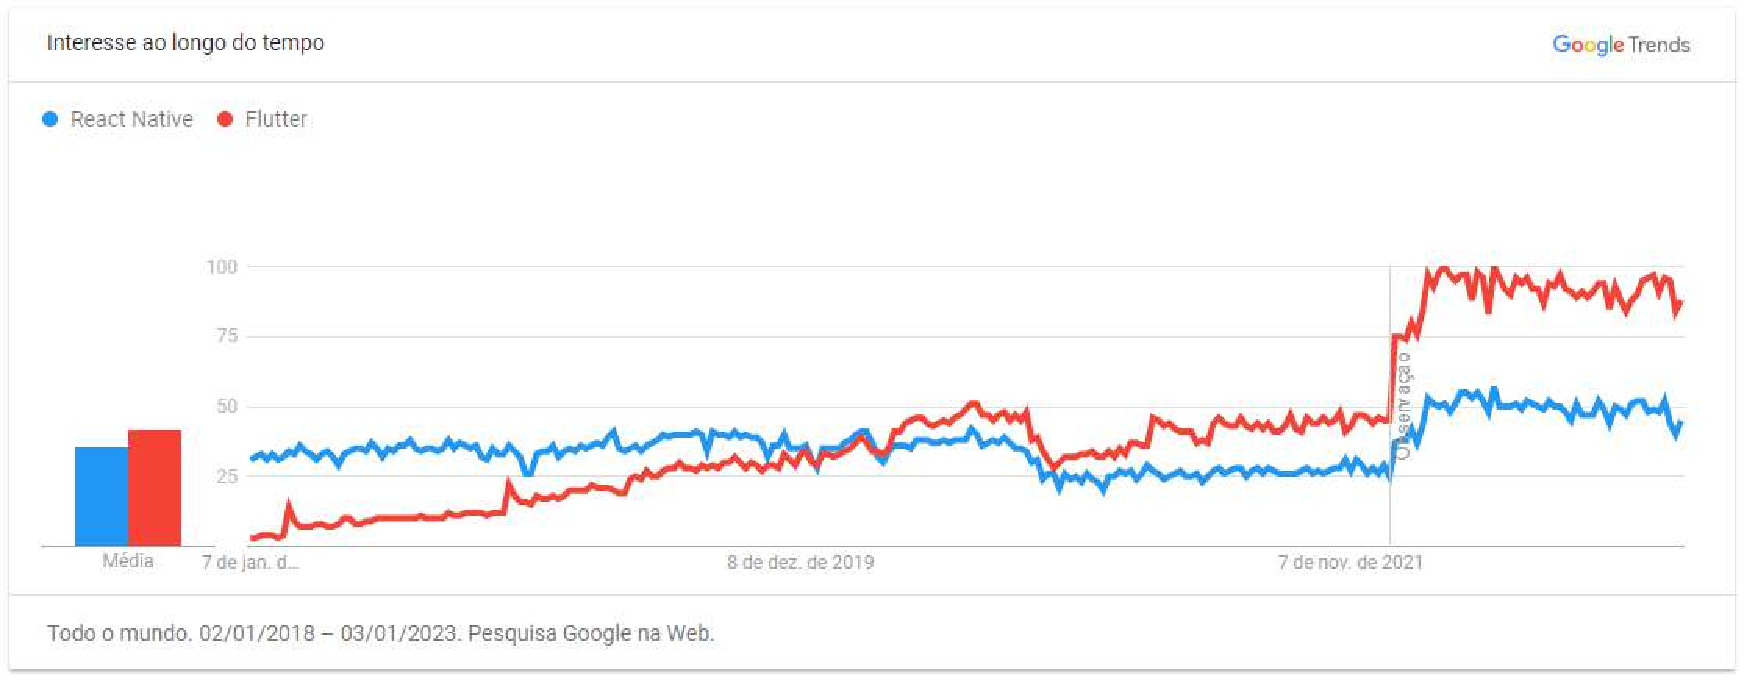
\includegraphics[width=\columnwidth]{images/interesse_flutter_react.pdf}
  \caption{Tendência mundial de popularidade do Flutter (vermelho) e do React Native (azul) (2018–2023).}
  \acsfont{Fonte: Google Trends\footref{google_trends_flutter_react}}
  \label{fig:interesse_flutter_react}
\end{figure}

Como explicado na página oficial sobre a arquitetura do Flutter\footnote{\label{flutter_arch}Visão geral da arquitetura do Flutter: \url{https://docs.flutter.dev/resources/architectural-overview}}, a mesma é dividida em três camadas: o \textit{Framework}, \textit{Engine} e o \textit{Embedder}. Ele existe como uma série de bibliotecas independentes, cada uma dependendo da camada subjacente. 

\begin{figure}[H]
\centering
  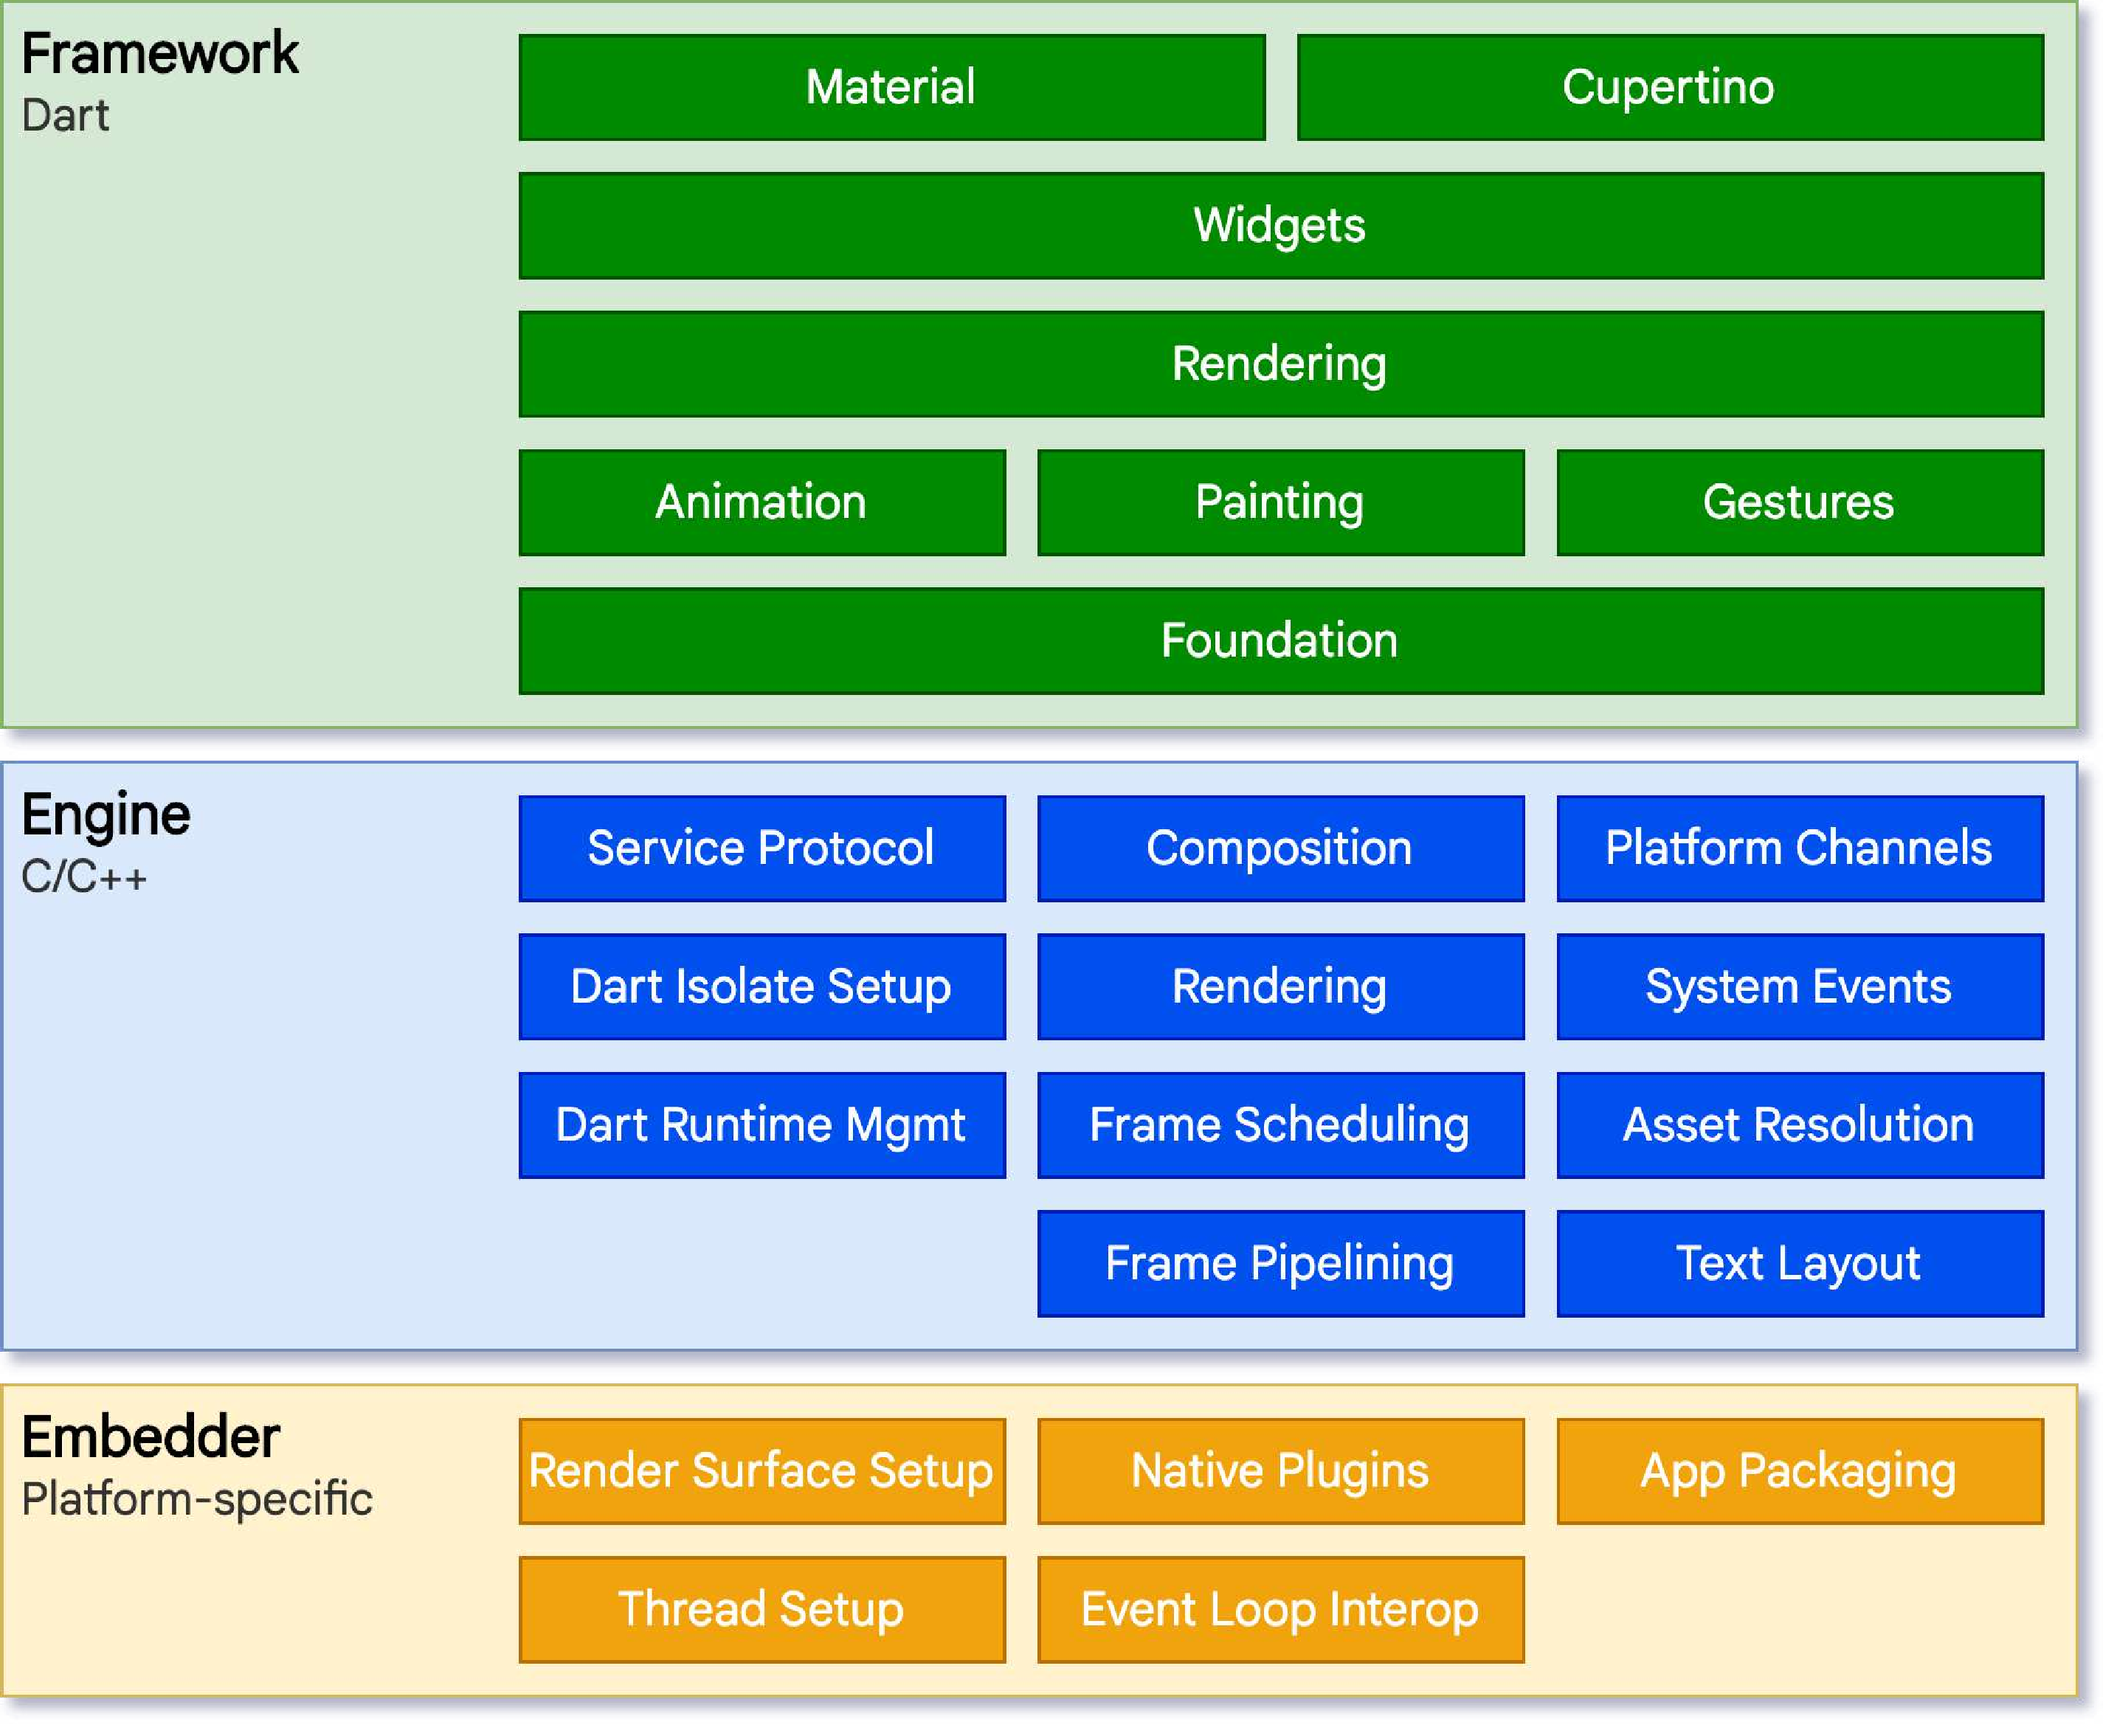
\includegraphics[width=\columnwidth]{images/flutter-archdiagram.pdf}
  \caption{Visão geral da arquitetura do Flutter.}
  \acsfont{Fonte: Flutter\footref{flutter_arch}}
  \label{fig:flutter-archdiagram}
\end{figure}

De forma resumida, a camada do \textit{framework} é moderna e reativa, escrito na linguagem \textit{Dart}, ela fornece uma \ac{api} de nível superior para criar \acp{app} de alta qualidade (por exemplo, \textit{widgets}, teste de cliques, detecção de gestos, acessibilidade, entrada de texto). Já a camada de \textit{engine} é escrita em \textit{c++} e fornece implementação de baixo nível das principais APIs do Flutter. Por fim o \textit{embedder} é o responsável por fornecer um ponto de entrada para aplicações e por coordenar acesso aos serviços dos \acp{so} como superfícies de renderização, acessibilidade e entrada, gerenciando o \textit{loop} de eventos de mensagens.

Outro ponto levado em consideração para a escolha do Flutter para o projeto, que também é um reflexo de seu crescimento, é que o mesmo se tornou um \textit{framework} multiplataforma muito poderoso, que, segundo o site oficial do Flutter\footnote{Flutter: \url{https://flutter.dev/multi-platform}} atualmente permite ser compilado para aplicações web, desktop (MacOS, Windows e Linux), dispositivos móveis (Android e iOS) e até dispositivos embarcados a partir de um mesmo código fonte. Desta forma, sendo possível expandir futuramente este projeto para uma ampla gama de dispositivos além dos \acp{dm}.

\section{Código Limpo}\label{sec:codigo_limpo}
O projeto foi desenvolvido usando as técnicas e referencias do livro "Código Limpo: Habilidades Práticas do \textit{Agile Software}", publicado em 2008, por Robert C. Martin, também conhecido como "\textit{Uncle Bob}" ou em português "Tio Bob", a seguir, uma breve definição: O Código Limpo é um conjunto de práticas e princípios para escrever código de alta qualidade, fácil de entender e manter. Essa abordagem de programação foi popularizada pelo Tio Bob, em seu livro acima citado.

Um código limpo deve ser legível, expressivo, ter baixa complexidade, ser fácil de testar e modular \cite{martin2008codigolimpo}. Além disso, ele deve seguir princípios citados como "S.O.L.I.D.", um acrônimo criado por Michael Feathers que representa os 5 princípios da programação orientada a objetos.

“Os programas escritos nessas linguagens podem parecer estruturados e orientados a objetos, mas a aparência pode enganar. Com muita frequência, os programadores de hoje desconhecem os princípios que são a base das disciplinas das quais suas linguagens foram derivadas. [...] Esses princípios expõem os aspectos de gerenciamento de dependência do design orientado a objetos em oposição aos aspectos de conceituação e modelagem. Isso não quer dizer que a OO seja uma ferramenta ruim para a conceituação do espaço do problema ou que não seja um bom local para a criação de modelos. Certamente muitas pessoas obtêm valor desses aspectos da OO. Os princípios, no entanto, concentram-se fortemente no gerenciamento de dependências.” \cite{martin2005principles}.

A seguir, os cinco princípios abordados a serem seguidos para a criação de um bom código:
\begin{enumerate}
    \item \textbf{SRP} - Princípio da Responsabilidade Única (\textit{Single Responsibility Principle}): Uma classe deve ter um, e somente um, motivo para mudar.
    \item \textbf{OCP} - Princípio do Aberto/Fechado (\textit{Open/Closed Principle}): Você deve ser capaz de estender um comportamento de uma classe sem a necessidade de modificá-lo.
    \item \textbf{LSP} - Princípio da Substituição de Liskov (\textit{Liskov Substitution Principle}): As classes derivadas devem ser substituíveis por suas classes bases.
    \item \textbf{ISP} - Princípio da Segregação de Interfaces (\textit{Interface Segregation Principle}): Muitas interfaces específicas são melhores do que uma interface única geral.
    \item \textbf{DIP} - Princípio da Inversão de Dependência (\textit{Dependency Inversion Principle}): Dependa de abstrações e não de implementações.
\end{enumerate}

A aplicação desses princípios e práticas de código limpo pode levar a benefícios como redução do tempo de desenvolvimento, maior facilidade de manutenção, maior eficiência e redução de bugs. O que foi notado no desenvolvimento deste projeto.


\section{Arquitetura Limpa}\label{sec:arquitetura_limpa}
A chamada Arquitetura Limpa ou \textit{Clean Architecture} é um tema bastante abordado atualmente na área de desenvolvimento de \textit{software}. Esse conceito também foi criado por Robert C. Martin e tem como objetivo principal a criação de sistemas de \textit{software} de alta qualidade, duráveis e que possam ser facilmente modificados e mantidos. A Arquitetura Limpa é baseada em três princípios fundamentais: separação de interesses, independência de \textit{frameworks} e testabilidade \cite{martin2018arquitetura}.

A separação de interesses é um dos pilares da Arquitetura Limpa. Ela se baseia na ideia de que as diferentes camadas de uma aplicação devem ser isoladas umas das outras, permitindo que cada uma delas possa ser modificada sem afetar as demais. Essa separação pode ser feita de diversas formas, mas é comum a utilização de padrões como o MVC (Model-View-Controller), MVVM (Model-View-ViewModel) e MVP (Model-View-Presenter).

A independência de frameworks também é um conceito importante na Arquitetura Limpa. De acordo com o Tio Bob, os \textit{frameworks} devem ser vistos como detalhes de implementação e não como parte da arquitetura. Isso significa que o código deve ser escrito de forma a não depender diretamente de nenhum \textit{frameworks} específico, facilitando a migração para outros \textit{frameworks} ou até mesmo para outras plataformas.

Por fim, a testabilidade é um princípio fundamental na Arquitetura Limpa. Segundo Martin, o código deve ser escrito de forma a ser facilmente testado, permitindo que os testes sejam executados com rapidez e eficiência. Para isso, é importante que as diferentes camadas da aplicação estejam bem separadas, permitindo que cada uma delas possa ser testada de forma independente.

\section{Engenharia de requisitos}\label{sec:eng_req}
A engenharia de requisitos é um processo fundamental na concepção e construção de sistemas, pois busca definir os requisitos do sistema em conjunto com os \textit{stakeholders}, produzindo uma série de artefatos em suas fases de concepção. 

Segundo \cite{kotonya1998requirements}, a engenharia de requisitos é o processo de descobrir, analisar, documentar e verificar serviços e restrições para um sistema. Embora não haja uma maneira irrefutável de garantir que as especificações construídas pela engenharia de requisitos sejam totalmente compatíveis com as necessidades dos \textit{stakeholders} e atendam às suas necessidades, este é o maior desafio encontrado na engenharia de requisitos \cite{pressman2016engenharia}. 

As etapas da engenharia de requisitos incluem a concepção e análise de requisitos, levantamento e compreensão dos requisitos junto ao cliente, negociação dos requisitos, especificação e modelagem desses requisitos, tendo como objetivo documentar as necessidades e os propósitos do software.

\section{Requisitos funcionais de um software}\label{sec:req_func}
Segundo \cite{pressman2016engenharia}, os requisitos funcionais, que descrevem as funções e serviços que o software deve oferecer, descrevem como o software deve funcionar, quais entradas devem ser processadas e quais saídas devem ser geradas em resposta a essas entradas. 

\section{Casos de uso de um software}\label{sec:req_func}
Os Casos de Uso (\textit{Use Cases}) são uma técnica de modelagem de requisitos de software que descrevem as interações entre o usuário e o sistema. Eles ajudam a identificar as funcionalidades e serviços que o software deve oferecer, além de fornecer um meio de comunicação claro entre as equipes de desenvolvimento e os \textit{stakeholders}, como aborda \cite{martin2008agile}.

\section{Prototipação}\label{sec:prototipacao}
\cite{warfel2009prototyping} destaca que os protótipos de baixa fidelidade são rápidos e baratos de criar, permitindo que os \textit{designers} testem e refinem rapidamente ideias iniciais. Já os protótipos de alta fidelidade, embora mais caros e demorados, podem ajudar a obter \textit{feedback} mais preciso e detalhado sobre o \textit{design} e a usabilidade do software.

\section{Desenvolvimento de sistemas}\label{sec:dev_sistemas}
O desenvolvimento de sistemas é um processo que envolve diversas etapas, desde a concepção do projeto até a entrega do produto final. Segundo \cite{pressman2016engenharia}, a fase de análise de requisitos é fundamental para entender as necessidades do cliente e garantir que o sistema desenvolvido atenda às expectativas. 

Já \cite{somerville2015engenharia} destaca a importância da fase de design na criação de uma arquitetura que atenda aos requisitos do sistema, bem como na escolha de tecnologias e ferramentas adequadas para a implementação. Além disso, o processo de teste é fundamental para garantir a qualidade do sistema desenvolvido, de acordo com \cite{myers2012art}. 

Por fim, é importante ressaltar que o desenvolvimento de sistemas é uma área em constante evolução e que novas metodologias e práticas surgem frequentemente, como o desenvolvimento ágil, conforme destacado por \cite{martin2008agile}.
\subsection{Metodologias ágeis}\label{ssec:metodologias_ageis}
As metodologias ágeis são uma abordagem de desenvolvimento de \textit{software} que prioriza a interação contínua com o cliente, adaptação rápida às mudanças e entrega frequente de funcionalidades em pequenos incrementos. Essas metodologias se baseiam em valores e princípios que enfatizam a colaboração, o trabalho em equipe, a comunicação constante e a flexibilidade, em contraste com as abordagens mais tradicionais que tendem a ser mais burocráticas e hierárquicas. 

As metodologias ágeis se tornaram cada vez mais populares nos últimos anos, principalmente devido à sua eficácia em projetos complexos e dinâmicos, bem como ao seu foco no valor entregue ao cliente. A seguir, uma breve explicação sobre duas metodologias que foram mutualmente aplicadas no desenvolvimento do sistema.
\subsubsection{Scrum}\label{sssec:scrum}
O Scrum é uma metodologia ágil baseada em uma estrutura de trabalho em equipe que divide o projeto em sprints, ciclos de tempo definidos, com objetivos claros e bem definidos. Durante cada sprint, a equipe trabalha em conjunto para atingir esses objetivos, fazendo ajustes e melhorias ao longo do caminho. As equipes de desenvolvimento são auto-organizadas e multidisciplinares, o que permite que cada membro tenha uma visão ampla do projeto e possa contribuir com suas habilidades e experiências específicas. Além disso, a metodologia promove a comunicação constante entre as equipes, com reuniões diárias para acompanhar o progresso e identificar possíveis problemas.

\begin{figure}[h]
\centering
  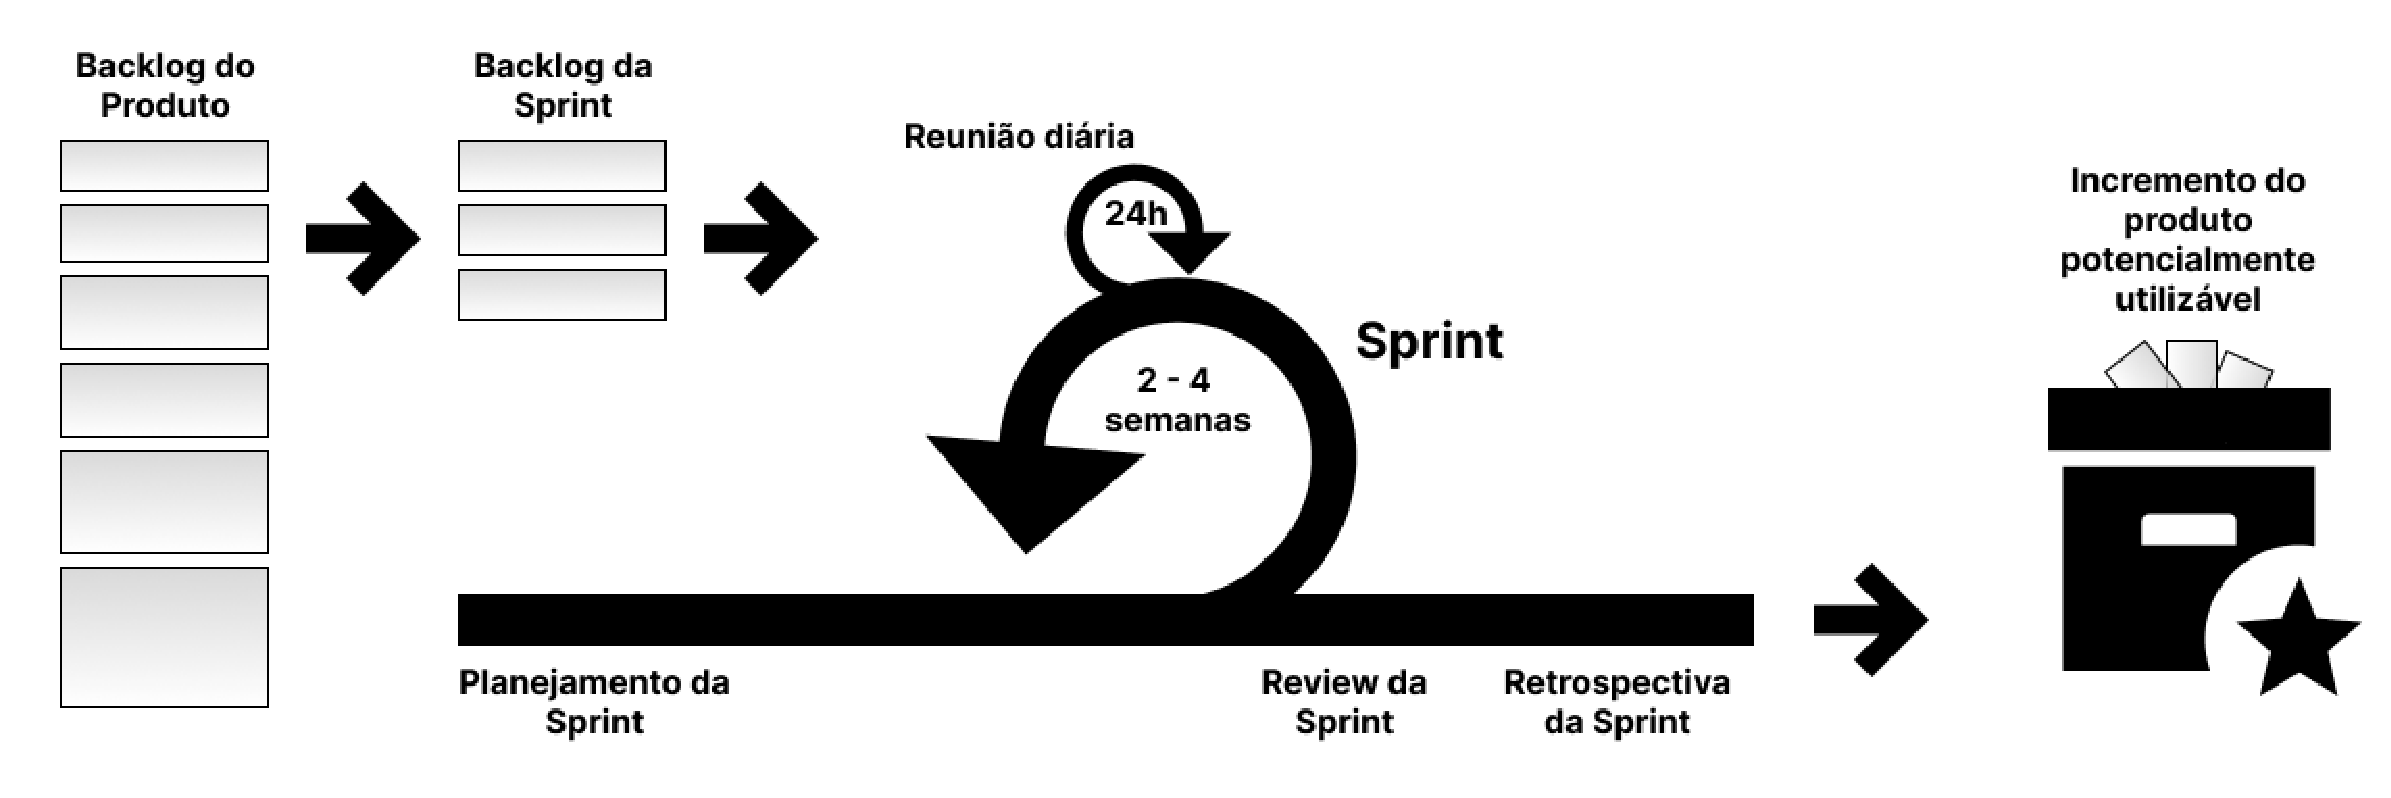
\includegraphics[width=\columnwidth]{images/scrum.pdf}
  \caption{Representação de uma Sprint com o framework Scrum.}
  \acsfont{Fonte: Adaptação de \cite{sutherland2014scrum}}
  \label{fig:scrum}
\end{figure}

De acordo com o processo ágil do Scrum, existem cinco eventos (também chamados de cerimônias). São eles:

\begin{enumerate}
    \item Reunião de planejamento (\textit{Planning Meeting}): Para determinar o que pode ser entregue na Sprint que se inicia, e como o trabalho será feito.
    \item Reunião diária (\textit{Daily Scrum}): Realiza-se uma reunião de no máximo 15 minutos, idealmente no mesmo horário, nesta reunião o time inspeciona rapidamente seu trabalho e planeja o trabalho a ser feito para as próximas 24 horas.
    \item Reunião de revisão da Sprint (\textit{Sprint Review}): Ocorre tipicamente no último dia. Ela tem como objetivo inspecionar as entregas feitas pelo time durante a Sprint e adaptar o backlog do produto se necessário.
    \item Reunião de retrospectiva da Sprint (\textit{Sprint Retrospective}): Nesta reunião o time expõe de forma bastante transparente o que está funcionando e o que deve ser melhorado na maneira que o time está trabalhando.
    \item A Sprint em si, a qual engloba os demais eventos acima.
\end{enumerate}

\subsubsection{Kanban}\label{sssec:kanban}
O Kanban é uma metodologia ágil que surgiu no Japão, em meados da década de 1940, com o objetivo de aumentar a eficiência do processo produtivo nas fábricas da Toyota. O método baseia-se na visualização do fluxo de trabalho por meio de um quadro Kanban, que mostra as tarefas a serem realizadas, em andamento e concluídas, permitindo que a equipe visualize o processo e identifique gargalos e desperdícios. 

É comum acharem que o Kanban é uma ferramenta do Scrum, o que e não é verdade, ele nada mais é que uma ferramenta que vai ajudar o Scrum a ser mais eficaz no controle da quantidade de trabalho em progresso. Hoje ele vem sendo utilizando largamente no desenvolvimento de \textit{software}, e com sua adoção em projetos de \textit{software}, tem-se um processo mais transparente, colaborativo e ágil, possibilitando um melhor gerenciamento do trabalho em equipe.

\begin{figure}[h]
\centering
  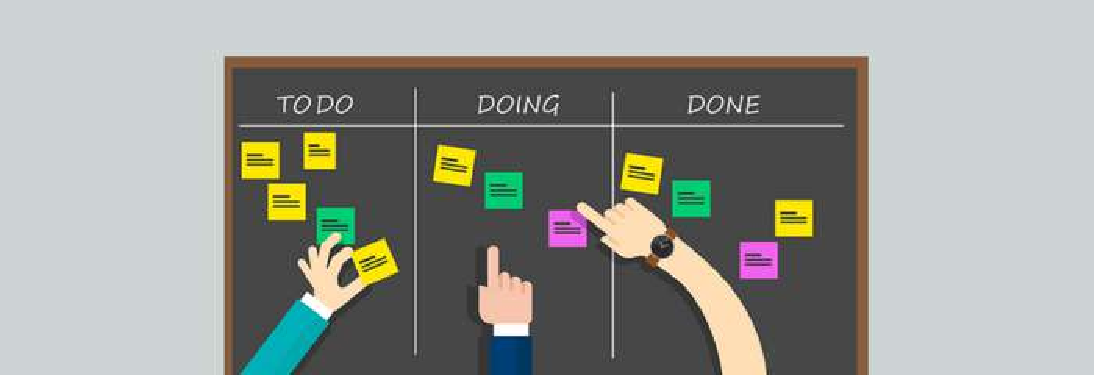
\includegraphics[width=\columnwidth]{images/kanban.pdf}
  \caption{Representação de um quadro de desenvolvimento com o framework Kanban.}
  \acsfont{Fonte: \cite{metodoagilKanban}}
  \label{fig:kanban}
\end{figure}

O quadro geralmente é autoexplicativo, suas colunas são flexíveis, sendo adaptadas de acordo com o uso, mas existem pelo menos três, são elas:

\begin{enumerate}
    \item Para fazer (\textit{TODO}): Tarefas pendentes.
    \item Fazendo (\textit{Doing}): Tarefas em progresso.
    \item Feito (\textit{Done}): Tarefas concluídas.
\end{enumerate}

\section{Prototipagem}\label{sec:prototipagem}
A prototipagem é uma técnica importante no processo de desenvolvimento de \textit{software}, permitindo aos desenvolvedores criar modelos iniciais do produto para avaliar e testar sua funcionalidade e usabilidade, essencial na construção de um \ac{mvp}. Ao criar protótipos, os desenvolvedores podem obter feedback dos usuários e identificar problemas com antecedência, o que pode ajudar a evitar atrasos e aumentar a satisfação do cliente. De acordo com \cite{fidel2003user}, a prototipagem é considerada uma das práticas mais importantes no design de interação, ajudando a reduzir os custos de desenvolvimento e melhorar a eficiência do processo de design.

Neste projeto, a ferramenta de prototipagem utilizada majoritariamente foi o Figma, que será explicado na subseção abaixo.
\subsection{Figma}\label{ssec:figma}
O Figma é uma das diversas ferramentas de prototipagem de interfaces de usuário existente e é amplamente utilizada em projetos de desenvolvimento de \textit{software}. Sua interface intuitiva e recursos colaborativos facilitam a criação de protótipos interativos, que permitem aos designers e desenvolvedores visualizar como o produto final funcionará. Ele também oferece recursos de design, como a criação de ícones, gráficos e wireframes, permitindo que os designers criem designs personalizados e aprimorem a aparência geral do produto. 

Além disso, o Figma suporta o compartilhamento de projetos, permitindo que vários membros da equipe colaborem em tempo real e facilitem a comunicação. Com esses recursos, ele tornou-se uma ferramenta valiosa para equipes de desenvolvimento de \textit{software} que buscam agilidade e eficiência no processo de prototipagem e design.

